%
% Documento: Trabalhos Relacionados
%

\chapter{Trabalhos Relacionados}

Na literatura, diversos são os exemplos de sistemas não lineares para os quais se desenvolvem diferentes tipos de controladores. Dentre estes tipos, encontramos os PD (Proporcional-Derivativo), PID (Proporcional-Integral-Derivativo), LQ (Linear-Quadrático), Fuzzy e ANFIS dentre outros sendo que este último tem se mostrado bastante presente para tentar atuar sobre diferentes tipos de sistemas.
%Controle Adaptativo L1

A grande quantidade de materiais propondo a implementação de controladores neuro-fuzzy se deve, em parte, ao fato de geralmente, para efetuar tal controle, não ser necessário se fazer uma modelagem matemática aprofundada do sistema que, em diversos casos, é de grande complexidade e, por isso, demandaria um grande esforço sendo que em muitos casos os resultados não seriam tão bons quanto os desejados além de oferecer ainda uma boa robustez ao controle.

Além do próprio controle de estabilidade de helicópteros quadrotores, podem-se encontrar exemplos de diversos sistemas que implementam controladores neuro-fuzzy. É o caso da implementação de um controlador para \textit{see and avoid\footnote{Ver e evitar, tradução nossa}} (referente ao desvio de ocasionais obstáculos) de um \textit{drone}, como se pode encontrar em \citeonline{Olivares-Mendez2012}.

Já \citeonline{Guo2003}, propõem a implementação de um controlador neuro-fuzzy para controlar a estabilidade sobre o balanço de um barco. Os autores mostraram, ainda, que o controlador neuro-fuzzy obteve melhor resultado do que um controlador PID, chegando à conclusão de que controladores neuro-fuzzy são promissores para efetuar tal controle.

A grande gama de opções de controle sobre quadrotores pode ser dividida em dois grupos principais: o controle \textit{tradicional} e o controle \textit{inteligente}. O primeiro diz respeito ao uso de técnicas consolidadas para controle baseado na atuação sobre eles a partir do conhecimento de sua modelagem, ao passo que o segundo se refere às técnicas de controle que envolvem componentes de Inteligência Computacional, agregando, por exemplo, representação de estados através de variáveis linguísticas e capacidade de aprendizagem.

%\section{Controle de Estabilidade de um Pêndulo Invertido}
%\label{sec:trab-rel-pendulo-invetido}
%
%Um dos sistemas dinâmicos não lineares intrinsecamente instáveis mais estudados é o de pêndulo invertido, sendo comumente usado em \textit{benchmarks} para verificar a eficácia de métodos de controle. 

%Outro caso em que se é muito comum a implementação deste tipo de controlador é para o controle de estabilidade de um pêndulo invertido. Diversas são as abordagens que se encontram na literatura.
%Um pêndulo invertido é um sistema instável não linear comumente usado em \textit{benchmarks} para verificar a eficácia de métodos de controle. 
%A figura \autoref{fig:inverted-pendulum-diagram} ilustra o modelo de um pêndulo invertido. Este sistema é composto de uma barra rígida colocada verticalmente sobre um carro. O objetivo do sistema é manter a barra em equilíbrio oscilatório, fazendo com que ela não caia \cite{Arai2014}.
\iffalse
\begin{figure}[!htb]
    \centering
    \caption{Modelo de um pêndulo invertido}
    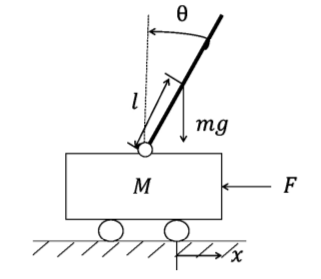
\includegraphics[width=0.4\textwidth]{./04-figuras/inverted-pendulum_diagram}
    \fonte{\cite[p.~416]{Arai2014}}
    \label{fig:inverted-pendulum-diagram}
\end{figure}

Na \autoref{fig:inverted-pendulum-diagram}, $M$ [$kg$] é a massa do carro, $m$ [$kg$] é a massa do pêndulo, $l$ [$m$] é metade do comprimento do pêndulo, $g$ [$m/s^2$] é a aceleração da gravidade e $\theta$ [$rad$] é o ângulo de desvio da barra em relação à posição vertical. O valor de cada variável de estado é calculada usando o método de Euller para um pequeno período de tempo $\tau$ [$s$].
\fi
\citeonline{Kim2000} compararam um controlador puramente LQR a um controlador híbrido, aliando o LQR a um controle neuro-fuzzy. A \autoref{fig:lqr-neuro-fuzzy-kim2000} mostra o esquema resultante. Neste modelo, a rede neural é configurada em paralelo ao controlador LQR. Este esquema consiste de um controlador LQR de ganho fixo que faz o sistema como um todo estável e um controlador realimentado que atualiza seus pesos internos para gerar o sinal de controle $u_{FN}$ contribuindo para a redução de tempo de convergência do sistema.

\begin{figure}[!htb]
    \centering
    \caption{Diagrama do controlador híbrido LQR-Neuro-Fuzzy implementado em \cite{Kim2000}}
    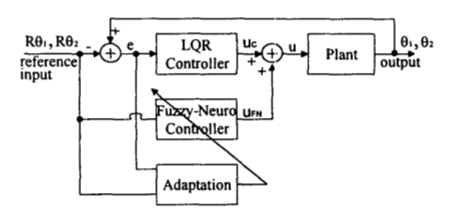
\includegraphics[width=0.6\textwidth]{./04-figuras/lqr_neuro_fuzzy_pendulum}
    \fonte{\cite[p.~416]{Kim2000}}
    \label{fig:lqr-neuro-fuzzy-kim2000}
\end{figure}

Resultados de simulação mostraram que o controlador híbrido LQR-Neuro-Fuzzy obteve menor erro na fase inicial de treinamento se comparado ao controlador LQR. Além disto, os resultados mostraram que o controlador proposto é mais eficiente que o LQR, obtendo melhor tempo de convergência.

\citeonline{Omatu1994} também propuseram um controlador híbrido aliando os controles LQR e Fuzzy. Neste caso, entretanto, os controladores operam em momentos diferentes. O controlador neuro-fuzzy atua sobre o sistema até que o pêndulo se aproxime da posição vertical. A partir de um ponto de referência, o controle passa a ser efetuado pelo controlador LQR. Neste caso, mais uma vez a inserção de um controle por neuro-fuzzy contribiu para a boa resposta do sistema.

Em \cite{Alata2001}, outro tipo de controlador híbrido LQR-Neuro-Fuzzy é proposto. Neste caso, os ganhos em diferentes regiões de operação são calculados usando o método LQR. Esses ganhos são tabulados com os estados correspondentes do ponto de operação. Então, um agrupamento subtrativo e o ANFIS são usados para contruir a base de dados e a base de regras do sistema de inferências fuzzy. Isto fornece um mecanismo suave de transição de um ponto de operação para outro. A eficácia da abordagem proposta foi provada por resultados experimentais de um pêndulo invertido.

Já \citeonline{Arai2014} utilizaram uma abordagem diferente, implementando um controlador puramente CVNF (\textit{Complex-Valued Neuro-Fuzzy}\footnote{Neuro-Fuzzy com Valores Complexos, tradução nossa}), que diz repeito a uma expansão de um controlador neuro-fuzzy para o conjunto dos números complexos. Algumas das vantagens deste método são que ele apresenta menor tempo de treinamento e, ainda assim, uma melhor precisão de treinamento. Utilizando-o, os autores obtiveram um resultado melhor do que usando um controlador Neuro-Fuzzy, possuindo melhor tempo de resposta e, ainda, um maior alcance de ângulos iniciais que podem ser compensados.


%\subsection{Métodos de Controle Tradicional de Helicópteros Quadrotores}
%\label{sec:trab-rel-quadrotores-sub-trad}
\section{Controle Tradicional de Quadrotores}
\label{sec:trab-rel-tradicional}

Esta seção aborda diferentes propostas de controladores tradicionais para quadricópteros visando a contextualização do estado da arte para depois se poder comparar alguns resultados das técnicas tradicionais e inteligentes de controle para esse sistema.

Em \cite{Razinkova2014}, foi proposto um controlador PD para a descrição adequada das trajetórias definidas de um quadricóptero \textit{Indoor}. Para permitir um funcionamento adequado \textit{Outdoor}, foi integrado ao controlador PD um controle adaptativo, adicionando termos ao controlador convencional, de forma a permitir o ajuste correto da trajetória do quadricóptero quando submetido a distúrbios nos eixos X e Y (plano horizontal). Os resultados mostraram que o controlador adaptativo melhorou consideravelmente o controle de trajetória do \textit{drone}, reduzindo em 64\% o erro de posicionamento para os casos de trajetória em linha reta ao longo do plano XY, e em 72\% para os casos de trajetória circular sobre o plano XY. Segundo os autores, este resultado representa uma melhora significativa, uma vez que o controlador resultante possui uma arquitetura simples e não requer computação extensiva, o que é indesejado para qualquer controle de sistema, especialmente para UAVs, devido à sua limitação de bateria.

Em \cite{Mustapa2014} é proposto um controlador PID para efetuar o controle visando a estabilidade da altitude de um quadricóptero. Neste trabalho, foi utilizado um modelo matemático desenvolvido previamente para descrever o comportamento do sistema. Para ajustar os parâmetros do controlador PID, foi necessário realizar um experimento para determinar o momento de inércia do drone. Uma vez levantados os valores necessários, um controlador PID foi ajustado e se mostrou eficiente. A simulação do sistema foi realizada no Matlab Simulink\textsuperscript{\textregistered}.

\citeonline{Khatoon2014} também propuseram um controlador PID para controlar a estabilidade em altitude de um drone, mantendo a posição no eixo XY constante, mesmo esta altitude sendo uma variável muito sensível a mudanças em outros parâmetros. No trabalho, é mostrado que um controlador PID sozinho é capaz de exercer tal controle com robustez. A escolha deste controlador se deu graças à sua robustez e facilidade de modelagem. Entretanto, é também apontado pelos autores que, apesar da simplicidade para se modelar um controlador PID, isto requer uma modelagem do sistema como um todo, o que não é fácil, devido à sua estrutura complexa, suas dinâmicas não lineares e sua natureza subatuada. O sistema modelado para o drone mostrou ser altamente instável, justificando a necessidade de um controlador. A partir de extensivas simulações no MATLAB/Simulink, o sistema desenvolvido se mostrou bem sucedido, implementando de fato um controle robusto de altitude para um helicóptero quadricóptero.

Além desses controladores que aplicam técnicas tradicionais, são também vários os exemplos de trabalhos que exploram o controle inteligente de quadricópteros.

%\subsection{Métodos de Controle Inteligente de Helicópteros Quadrotores}
%\label{sec:trab-rel-quadrotores-sub-ia}
\section{Controle Inteligente de Quadrotores}
\label{sec:trab-rel-inteligenge}

Além das técnicas de controle tradicionais, encontram-se também na literatura diversas abordagens para a construção de controladores de estabilidade para \textit{drones} utilizando técnicas da Inteligência Computacional. As propostas vão do uso de algoritmos de otimização (e.g.\ algoritmos genéticos, PSO) ao uso de sistemas neuro-\textit{fuzzy} expandido para o espaço dos números complexos.

%22
%\cite{Rezazadeh2013}
Em \cite{Rezazadeh2013}, é proposto um controlador neuro-\textit{fuzzy} (ANFIS) para o controle estabilizante de altitude de um quadricóptero. O módulo \textit{fuzzy} acoplado a um controlador PID é usado para controlar a atitude. Os controladores \textit{fuzzy} atualizam os ganhos do PID \textit{online} para produzir uma resposta apropriada. A saída é calculada diretamente pelo ajuste dos pesos das entradas de acordo com as regras de inferência \textit{fuzzy}. Estas regras, que são a base de conhecimento, são determinadas por um algoritmo computacional baseado em redes neurais. O controlador proposto foi comparado a um simples controlador PID e, a partir de simulações, foi mostrado que se obteve melhor resposta, por exemplo, tendo em vista o tempo de assentamento e a sobrelevação. Outro resultado obtido foi de que o controlador ANFIS é capaz de estabilizar o sistema quando exposto a perturbações externas.

%34
%\cite{Mahfouz2013}
Em \cite{Mahfouz2013}, foi proposto um controlador parecido. Neste trabalho, também foi sugerido um controlador ANFIS que, juntamente com um algoritmo genético, ajusta os pesos de um controlador PID. Mais uma vez, foi obtido sucesso com o controlador desenvolvido, sendo possível garantir a estabilidade de um \textit{drone} mesmo quando sujeito a perturbações. No trabalho, foi mostrado que a sobrelevação do controlador ANFIS é menor do que a do PID. Além disto, o erro de regime permanente no caso do ANFIS é zero, enquanto, no caso do controaldor PID, não o é. Uma conclusão muito importante a que se chega é que, do ponto de vista de robustez, os dois controladores são efetivos; do ponto de vista de performance, o ANFIS é melhor que o PID.

%14
%\cite{Maj2013}
Em \cite{Maj2013} é proposto um controle de estabilidade para um quadricóptero usando lógica \textit{fuzzy}. Neste trabalho, três controladores \textit{fuzzy} são usados: um para cada um dos dois eixos horizontais (\textit{x} e \textit{y}) e mais um controlador geral para todo o sistema. Com isto, o erro angular e a aceleração são as variáveis linguísticas. Em ambos os casos, são usados cinco termos linguísticos: muito negativo (NL), pouco negativo (NS), zero (Z), pouco positivo (PS) e muito positivo (PL). Os conjuntos NS, Z e PS são triangulares enquanto os conjuntos NL e PL são trapezoidais, como mostra a Figura \ref{fig:Maj2013_fuzzy_sets}. 

\begin{figure}[!htb]
    \centering
    \caption{Conjuntos \textit{fuzzy} usados em \cite{Maj2013}; a) erro de posição; b) erro de giro }
    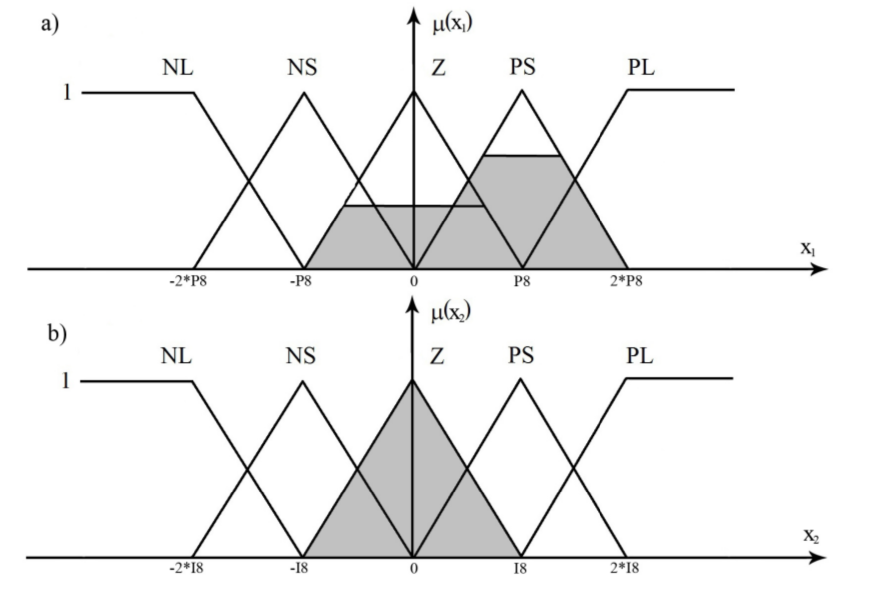
\includegraphics[width=0.6\textwidth]{./04-figuras/Maj2013_fuzzy_sets}
    \fonte{\cite{Maj2013}}
    \label{fig:Maj2013_fuzzy_sets}
\end{figure}

O bloco de fuzzificação calcula o grau de confiança dos conjuntos de entrada e um segundo bloco executa a inferência, que calcula o grau de confiança dos conjuntos de saída. As operações MIN e MAX são usadas como operadores AND e OR respectivamente para os conjuntos \textit{fuzzy}. O conjunto de regras utilizadas é mostrado no Quadro \ref{qua:Maj2013_table_rules_inference}.
% e os conjuntos \textit{fuzzy} antes da defuzzificação são mostrados na Figura \ref{fig:Maj2013_fuzzy_sets_output}.

\begin{quadro}[!htb]
    \centering
    \caption{Regras de inferência fuzzy usadas em \cite{Maj2013}\label{qua:Maj2013_table_rules_inference}}
    % \begin{tabular}{|p{3cm}|p{3cm}|p{3cm}|p{3cm}|p{3cm}|p{3cm}|}
    \begin{tabular}{c|c|c|c|c|c|}
        \cline{2-6}
        & \multicolumn{5}{c|}{\textbf{Erro de Giro}} \\
        
        \hline
        \multicolumn{1}{ |c| }{\textbf{Erro Angular}} & 
                            \textbf{NL} &
                            \textbf{NS} & 
                            \textbf{Z}  & 
                            \textbf{PS} & 
                            \textbf{PL}  \\
        \hline
        \multicolumn{1}{ |c| }{\textbf{NL}} & 
                            PL &
                            PL & 
                            PL & 
                            PS & 
                            Z  \\
        \hline
        \multicolumn{1}{ |c| }{\textbf{NS}} & 
                            PL &
                            PL & 
                            PS & 
                            Z  & 
                            NS \\

        \hline
        \multicolumn{1}{ |c| }{\textbf{Z}} & 
                            PL &
                            PS & 
                            Z  & 
                            NS & 
                            NL \\
        \hline
        \multicolumn{1}{ |c| }{\textbf{PS}} & 
                            PS &
                            Z  & 
                            NS & 
                            NL & 
                            NL \\
        \hline
        \multicolumn{1}{ |c| }{\textbf{PL}} & 
                            Z  &
                            NS & 
                            NL & 
                            NL & 
                            NL \\
        \hline
    \end{tabular}
    \fonte{Adaptado de \citeonline{Maj2013}}
\end{quadro}












% \begin{quadro}[!htb]
%     \centering
%     \caption{Tabela de regras para inferência.\label{qua:Maj2013_table_rules_inference}}
%     % \begin{tabular}{|p{3cm}|p{3cm}|p{3cm}|p{3cm}|p{3cm}|p{3cm}|}
%     \begin{tabular}{c|c|c|c|c|c|}
%         \cline{2-6}
%         & \multicolumn{5}{c|}{\textbf{Erro de Giro}} \\
%         % \cline{2-6}
        
%         \hline
%         \multicolumn{1}{ |c| }{\textbf{Erro Angular}} & 
%                             \textbf{NL} &
%                             \textbf{NS} & 
%                             \textbf{Z} & 
%                             \textbf{PS} & 
%                             \textbf{PL} \\
%         \hline
%             % \textbf{Erro Angular} & 
%             % \textbf{NL} &
%             % \textbf{NS} & 
%             % \textbf{Z} & 
%             % \textbf{PS} & 
%             % \textbf{PL} \\
%         % \hline
%         % a & b & c & d & e & f \\
%         % \hline
%     \end{tabular}
%     \fonte{Adaptado de \citeonline{Maj2013}}
% \end{quadro}

















%backup
% \begin{quadro}[!htb]
%     \centering
%     \caption{Tabela de regras para inferência.\label{qua:Maj2013_table_rules_inference}}
%     % \begin{tabular}{|p{3cm}|p{3cm}|p{3cm}|p{3cm}|p{3cm}|p{3cm}|}
%     \begin{tabular}{|c|c|c|c|c|c|}
%         \hline
%             \textbf{Erro Angular/Erro de Giro} & 
%             \textbf{NL} &
%             \textbf{NS} & 
%             \textbf{Z} & 
%             \textbf{PS} & 
%             \textbf{PL} \\
%         \hline
%         a & b & c & d & e & f \\
%         \hline
%     \end{tabular}
%     \fonte{Adaptado de \citeonline{Maj2013}}
% \end{quadro}



%\begin{figure}[!htb]
%    \centering
%    \caption{Conjuntos fuzzy antes da defuzzificação usados em \cite{Maj2013} }
%    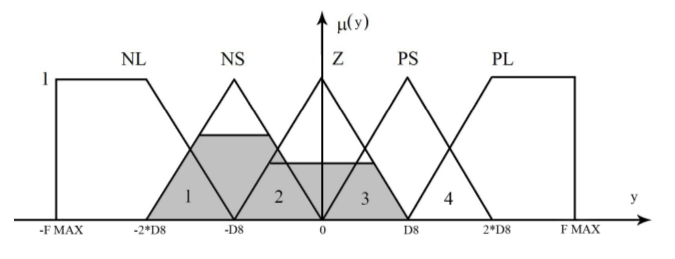
\includegraphics[width=0.6\textwidth]{./04-figuras/Maj2013_fuzzy_sets_output}
%    \fonte{\cite{Maj2013}}
%    \label{fig:Maj2013_fuzzy_sets_output}
%\end{figure}

Os autores obtiveram sucesso no controle estabilizante do \textit{drone}, mas somente utilizando um bloco integrador. Apesar de os reguladores e motores serem do mesmo tipo, algumas características deles são levemente diferentes. Como consequência, os motores não giram todos na mesma velocidade causando uma inclinação do quadricóptero. Esta inclinação pode ser corrigida com o uso de um bloco integrador. Desta forma, foi observado que um controlador puramente \textit{fuzzy} pode não ser suficiente para lidar com esta situação mas que, acoplando um bloco integrador, o sistema certamente pode ser estabilizado.
%A solução encontrada foi, portanto, implementar um controlador híbrido, que se mostrou eficiente para tal propósito.

%06
%\cite{Coza2006}
\citeonline{Coza2006} propuseram um controlador \textit{fuzzy} adaptativo para controlar a estabilidade de um quadricóptero \textit{Outdoor}. A escolha deste tipo de controlador se deu graças a inconvenientes apresentados por outros métodos. Controle adaptativo pode ser apropriado, mas requer conhecimento aprofundado do tipo de não linearidades nas dinâmicas do sistema. Um SMC (\textit{Sliding Mode Control}\footnote{Controle por Modos Deslizantes (tradução nossa).}) pode ser apropriado mas pode causar chaveamento indesejado no sinal de controle. Sistemas de controle com RNAs podem ser apropriados, mas requerem intenso esforço computacional para operar.

A abordagem utilizada em \cite{Coza2006} se baseia na ideia de que diferentes conjuntos de centros de decodificação são capazes de aproximar uniformemente a mesma função não linear. Desta forma, é usado treino supervisionado sobre os centros alternados: o erro do estado treina o centro de controle e a diferença na saída treina os centros alternados. A partir de simulações, mostrou-se que o resultado obtido foi um controle estável, computacionalmente eficiente e teoricamente robusto a perturbações. Entretanto, em uma das situações de simulações de perturbações por vento, o controlador teve de sacrificar a bom desempenho computacional para prevenir o desvio de centro. Ainda assim, foi mostrado que um modelo \textit{fuzzy} adaptativo usando atualização de controle e centro pode ser usado para cada eixo de rotação: X, Y e Z. Para tanto, apenas quatro funções de pertinência Gaussianas foram usadas para cada entrada de controle.

%10
%\cite{Rabhi2011}
Em \cite{Rabhi2011} uma outra abordagem é utilizada. Neste caso, os autores propuseram um controlador Fuzzy TSK (Takagi-Sugeno-Kang) para controlar a estabilidade de um quadricóptero. O controlador foi modelado usando ferramentas matemáticas, mais especificamente LMIs (\textit{Linear Matrix Inequalities}\footnote{Desigualdades Matriciais Lineares (tradução nossa).}) e modelado empregando PDC (\textit{Parallel Distributed Compensation}\footnote{Compensação Paralela Distribuída (tradução nossa).}). O objetivo foi projetar um controlador fuzzy realimentado para garantir a estabilidade do sistema com robustez. Simulações mostram que o controlador projetado garante, de fato, a estabilidade global do sistema em malha fechada.

%13
%\cite{Sheikhpour2013}
\citeonline{Sheikhpour2013} seguiram a mesma linha de \citeonline{Rabhi2011} e propuseram um controlador fuzzy TSK para estabilização de altura de um quadricóptero. Mais uma vez, a técnica PDC foi utilizada para projetar o controlador de realimentação. Neste trabalho, entretanto, o controle de estabilidade levou em conta especificações de desempenho como taxa de decaimento e restrições na entrada. Como ambas condições podem ser representadas por LMIs, elas também foram usadas neste caso, sendo mais complexas por lidar com as restrições dadas. Foi mostrado que simultaneamente à resolução das LMIs, foi projetado não apenas um controlador \textit{fuzzy} estável mas também com inclusão de velocidade de resposta desejada e restrições na entrada de altitude no controlador. Os resultados obtidos em simulações mostram a viabilidade desta abordagem.

%16
%\cite{JavidiNiroumand2013}
\citeonline{JavidiNiroumand2013} propuseram uma forma alternativa de controlador também usando a lógica fuzzy. Na abordagem utilizada, primeiramente foi derivado um modelo dinâmico não linear de um quadricóptero e então foi desenvolvido um controlador híbrido usando métodos de controle tradicionais e inteligentes para estabilização de dinâmicas rotacionais. A técnica IBS (\textit{Integral Backstepping}) é um poderoso método de controle tradicional amplamente utilizado para tal tipo de sistema mas encontrar o coeficiente apropriado do algoritmo é um trabalho crítico. Neste caso, esse problema foi resolvido usando um método de controle \textit{fuzzy}. Foi mostrado nos resultados que o método IBS possui domínio de atração mais amplo em comparação a métodos de controle lineares como o PID e uma melhor convergência. Foi mostrado ainda que ambos controladores IBS e \textit{Fuzzy} IBS foram capazes de controlar o sistema de forma apropriada. Entretanto, o controlador FIBS (\textit{Fuzzy Integral Backstepping}) obteve resultados levemente superiores ao IBS além de ter apresentado benefícios como uma melhor rejeição a perturbações e melhor robustez.
%\footnote{\textit{Backstepping} Integral, tradução nossa}
%\footnote{Backstepping Integral Fuzzy, tradução nossa}

%20
%\cite{Ariffanan2014}
Já em \cite{Ariffanan2014}, foi proposto um controlador FSBC (\textit{Fuzzy Supervisory Backstepping Controller}\footnote{Controlador por \textit{Backstepping Fuzzy} Supervisionado (tradução nossa).}). O controlador projetado consiste em controlador de \textit{backstepping} que pode selecionar automaticamente seus parâmetros \textit{on line} por um mecanismo de supervisão \textit{fuzzy}. O critério de estabilidade para a estabilização do quadricóptero é provada pelo teorema de Lyapunov. Extensivas simulações mostram a eficácia desta abordagem, apontando que uma alta precisão no transiente e no tempo de controle foram alcançados. Além disto, os resultados indicam que a técnica proposta pode estabilizar quadricópteros com melhor desempenho se comparado a técnicas de estabilização lineares.

%
%19
%\cite{Gao2014Stability}
Em \cite{Gao2014Stability}, é proposto um outro tipo de controlador híbrido. Neste caso, o controle é feito a partir de um sistema composto por dois controladores independentes: um controlador \textit{Backstepping} e um segundo controlador \textit{Fuzzy} PID Adaptativo, que alia a lógica \textit{fuzzy} a um controlador PID. Quando o quadricóptero voa em boas condições, o controle de estabilidade é assumido pelo controlador \textit{Backstepping}. Quando o quadricóptero encontra vento ou outro fator de perturbação durante o voo, o controlador \textit{Fuzzy} PID Adaptativo\footnote{O controlador \textit{Fuzzy} PID Adaptativo é um controlador PID que emprega o Sistema de Inferência \textit{Fuzzy} (FIS) para ajustar os parâmetros $K_p$, $K_i$, $K_d$, ganhos proporcional, integral e derivativo respectivamente.} é usado para estabilizá-lo. . O controlador proposto alcançou sucesso nos testes realizados, permitindo que se complete a trajetória sem que perturbações afetem a precisão do controle. Com isso, o Sistema de Inferência \textit{Fuzzy} se mostrou eficiente para ajustar os ganhos do controlador PID de forma a possibilitar o controle eficiente do quadricóptero.

%A \autoref{fig:Gao2014Stability_block_diagram} mostra o diagrama de blocos representando o controlador Fuzzy PID.
%
%\begin{figure}[!htb]
%    \centering
%    \caption{Diagrama de blocos do controlador híbrido usando em \cite{Gao2014Stability}}
%    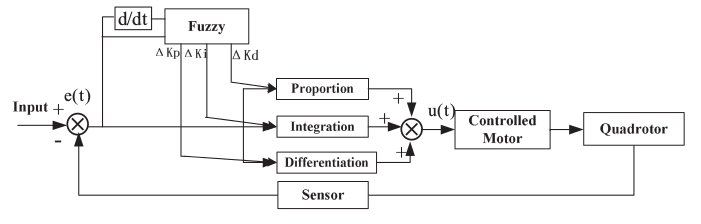
\includegraphics[width=0.9\textwidth]{./04-figuras/Gao2014Stability_block_diagram}
%    \fonte{\citeonline{Gao2014Stability}}
%    \label{fig:Gao2014Stability_block_diagram}
%\end{figure}
%
%Em relação à estrutura fuzzy, há duas entradas para a inferência fuzzy: o erro e a derivada do erro. São três saídas, cada uma sendo um parâmetro do controlador PID $\Delta kp$, $\Delta ki$ e $\Delta kd$. O universo de discurso foi normalizado e dividido em sete subconjuntos fuzzy. Os termos linguísticos foram definidos da seguinte forma: NB, negativo grande; NM, negativo médio; NS, negativo pequeno; ZO, aproximadamente zero; PS, positivo pequeno; PM, positivo médio; e PB, positivo grande. Os conjuntos fuzzy para cada variável de entrada consistem de sete variáveis linguísticas: $e$ = \{NB, NM, NS, ZO, PS, PM, PB\}, $e_c$ = \{NB, NM, NS, ZO, PS, PM, PB\}. As variáveis linguísticas das saídas são atribuídas da seguinte forma: $\Delta kp$ = \{ZO, PS, PM, PB\}, $\Delta ki$ = \{ZO, PS, PM, PB\}, $\Delta kp$ = \{ZO, PS, PM, PB\}. As regras de inferência Fuzzy para as variáveis de saída $\Delta kp$, $\Delta ki$ e $\Delta kd$ são mostradas nos Quadros \ref{qua:Gao2014Stability_table_rules_inference_kp}, \ref{qua:Gao2014Stability_table_rules_inference_ki} e \ref{qua:Gao2014Stability_table_rules_inference_kd} respectivamente.
%
%\begin{quadro}[!htb]
    \centering
    \caption{Regras de inferência fuzzy usadas em \cite{Gao2014Stability} para a variável $\Delta K_p$\label{qua:Gao2014Stability_table_rules_inference_kp}}
    \begin{tabular}{c|c|c|c|c|c|c|c|}
        \cline{2-8}
        & \multicolumn{7}{c|}{\textbf{$\Delta E_c$}} \\
        
        %cabeçalho
        \hline
        \multicolumn{1}{ |c| }{\textbf{E}} & 
                            \textbf{NB} &
                            \textbf{NN} & 
                            \textbf{NS} & 
                            \textbf{ZO} & 
                            \textbf{PS} & 
                            \textbf{PM} & 
                            \textbf{PB} \\
        \hline
        %NB OK
        \multicolumn{1}{ |c| }{\textbf{NB}} & 
                            PB &
                            PM &
                            ZO &
                            ZO &
                            ZO &
                            PM &
                            PB \\
        \hline
        %NM OK
        \multicolumn{1}{ |c| }{\textbf{NM}} & 
                            PB &
                            PM &
                            ZO &
                            ZO &
                            ZO &
                            PM &
                            PB \\
        \hline
        %NS OK
        \multicolumn{1}{ |c| }{\textbf{NS}} & 
                            PB &
                            PB &
                            PS &
                            ZO &
                            PS &
                            PB &
                            PB \\
        \hline
        %ZO OK
        \multicolumn{1}{ |c| }{\textbf{ZO}} & 
                            PB &
                            PB &
                            PS &
                            ZO &
                            PS &
                            PB &
                            PB \\
        \hline
        %PS OK
        \multicolumn{1}{ |c| }{\textbf{PS}} & 
                            PB &
                            PB &
                            PS &
                            ZO &
                            PS &
                            PB &
                            PB \\
        \hline
        %PM OK
        \multicolumn{1}{ |c| }{\textbf{PM}} & 
                            PB &
                            PM &
                            ZO &
                            ZO &
                            ZO &
                            PM &
                            PB \\
        \hline
        %PB OK
        \multicolumn{1}{ |c| }{\textbf{PB}} & 
                            PB &
                            PM &
                            ZO &
                            ZO &
                            ZO &
                            PM &
                            PB \\
        \hline

        % \multicolumn{1}{ |c| }{\textbf{NB}} & 
        %                     PB/ZO/PB &
        %                     PB/ZO/PB &
        %                     PB/ZO/PB &
        %                     PB/ZO/PB &
        %                     PB/ZO/PB &
        %                     PB/ZO/PB &
        %                     PB/ZO/PB \\
        % \hline

    \end{tabular}
    \fonte{Adaptado de \citeonline{Gao2014Stability}}
\end{quadro}






%
%\begin{quadro}[!htb]
    \centering
    \caption{Regras de inferência fuzzy usadas em \cite{Gao2014Stability} para a variável $\Delta K_i$\label{qua:Gao2014Stability_table_rules_inference_ki}}
    \begin{tabular}{c|c|c|c|c|c|c|c|}
        \cline{2-8}
        & \multicolumn{7}{c|}{\textbf{$\Delta E_c$}} \\
        
        %cabeçalho
        \hline
        \multicolumn{1}{ |c| }{\textbf{E}} & 
                            \textbf{NB} &
                            \textbf{NN} & 
                            \textbf{NS} & 
                            \textbf{ZO} & 
                            \textbf{PS} & 
                            \textbf{PM} & 
                            \textbf{PB} \\
        \hline
        %NB OK
        \multicolumn{1}{ |c| }{\textbf{NB}} & 
                            ZO &
                            ZO &
                            ZO &
                            PS &
                            ZO &
                            ZO &
                            ZO \\
        \hline
        %NM OK
        \multicolumn{1}{ |c| }{\textbf{NM}} & 
                            ZO &
                            ZO &
                            ZO &
                            PS &
                            ZO &
                            ZO &
                            ZO \\
        \hline
        %NS OK
        \multicolumn{1}{ |c| }{\textbf{NS}} & 
                            ZO &
                            ZO &
                            PS &
                            PS &
                            PS &
                            ZO &
                            ZO \\
        \hline
        %ZO OK
        \multicolumn{1}{ |c| }{\textbf{ZO}} & 
                            ZO &
                            ZO &
                            PS &
                            PS &
                            PS &
                            ZO &
                            ZO \\
        \hline
        %PS OK
        \multicolumn{1}{ |c| }{\textbf{PS}} & 
                            ZO &
                            ZO &
                            PS &
                            PS &
                            PS &
                            ZO &
                            ZO \\
        \hline
        %PM OK
        \multicolumn{1}{ |c| }{\textbf{PM}} & 
                            ZO &
                            ZO &
                            ZO &
                            PS &
                            ZO &
                            ZO &
                            ZO \\
        \hline
        %PB OK
        \multicolumn{1}{ |c| }{\textbf{PB}} & 
                            ZO &
                            ZO &
                            ZO &
                            PS &
                            ZO &
                            ZO &
                            ZO \\
        \hline

        % \multicolumn{1}{ |c| }{\textbf{NB}} & 
        %                     PB/ZO/PB &
        %                     PB/ZO/PB &
        %                     PB/ZO/PB &
        %                     PB/ZO/PB &
        %                     PB/ZO/PB &
        %                     PB/ZO/PB &
        %                     PB/ZO/PB \\
        % \hline

    \end{tabular}
    \fonte{Adaptado de \citeonline{Gao2014Stability}}
\end{quadro}






%
%\begin{quadro}[!htb]
    \centering
    \caption{Regras de inferência fuzzy usadas em \cite{Gao2014Stability} para a variável $\Delta K_d$\label{qua:Gao2014Stability_table_rules_inference_kd}}
    \begin{tabular}{c|c|c|c|c|c|c|c|}
        \cline{2-8}
        & \multicolumn{7}{c|}{\textbf{$\Delta E_c$}} \\
        
        %cabeçalho
        \hline
        \multicolumn{1}{ |c| }{\textbf{E}} & 
                            \textbf{NB} &
                            \textbf{NN} & 
                            \textbf{NS} & 
                            \textbf{ZO} & 
                            \textbf{PS} & 
                            \textbf{PM} & 
                            \textbf{PB} \\
        \hline
        %NB OK
        \multicolumn{1}{ |c| }{\textbf{NB}} & 
                            PB &
                            PB &
                            PM &
                            PS &
                            PM &
                            PB &
                            PB \\
        \hline
        %NM OK
        \multicolumn{1}{ |c| }{\textbf{NM}} & 
                            PB &
                            PB &
                            PM &
                            PS &
                            PM &
                            PB &
                            PB \\
        \hline
        %NS OK
        \multicolumn{1}{ |c| }{\textbf{NS}} & 
                            PB &
                            PM &
                            PS &
                            ZO &
                            PS &
                            PM &
                            PB \\
        \hline
        %ZO OK
        \multicolumn{1}{ |c| }{\textbf{ZO}} & 
                            PB &
                            PM &
                            PS &
                            ZO &
                            PS &
                            PM &
                            PB \\
        \hline
        %PS OK
        \multicolumn{1}{ |c| }{\textbf{PS}} & 
                            PB &
                            PM &
                            PS &
                            ZO &
                            PS &
                            PM &
                            PB \\
        \hline
        %PM OK
        \multicolumn{1}{ |c| }{\textbf{PM}} & 
                            PB &
                            PB &
                            PM &
                            ZO &
                            PM &
                            PB &
                            PB \\
        \hline
        %PB OK
        \multicolumn{1}{ |c| }{\textbf{PB}} & 
                            PB &
                            PB &
                            PM &
                            PS &
                            PM &
                            PB &
                            PB \\
        \hline

        % \multicolumn{1}{ |c| }{\textbf{NB}} & 
        %                     PB/ZO/PB &
        %                     PB/ZO/PB &
        %                     PB/ZO/PB &
        %                     PB/ZO/PB &
        %                     PB/ZO/PB &
        %                     PB/ZO/PB &
        %                     PB/ZO/PB \\
        % \hline

    \end{tabular}
    \fonte{Adaptado de \citeonline{Gao2014Stability}}
\end{quadro}







%O controlador proposto alcançou sucesso nos testes realizados, permitindo que se complete a trajetória sem que perturbações afetem a precisão de controle. O Sistema de Inferência \textit{Fuzzy} se mostrou eficiente para ajustar os ganhos do controlador PID de forma a possibilitar o controle eficiente do quadricóptero.

%28
%\cite{Gao2014Precision}
Em outro trabalho, os mesmos autores implementaram um outro controlador híbrido. Em \cite{Gao2014Precision}, foi proposto um controlador Fuzzy PD. Além disto, neste trabalho, são comparadas as performances de três controladores diferentes: PID, Fuzzy PD e \textit{Backstepping}. Mais uma vez, aqui o controlador fuzzy tem como função ajustar os parâmetros do controlador PD: $\Delta K_p$ e $\Delta K_d$.

A \autoref{fig:Gao2014Precision_block_diagram} mostra o diagrama de blocos do controlador neste caso. Como se pode ver, o diagrama mostra o controlador Fuzzy PD e um controlador PID.

\begin{figure}[!htb]
    \centering
    \caption{Diagrama de blocos do controlador híbrido usando em \cite{Gao2014Precision}}
    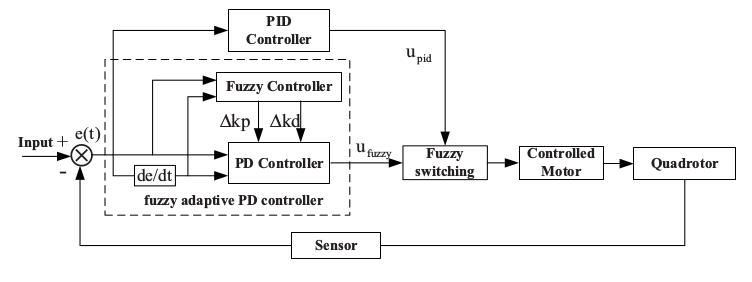
\includegraphics[width=0.9\textwidth]{./04-figuras/Gao2014Precision_block_diagram}
    \fonte{\citeonline{Gao2014Precision}}
    \label{fig:Gao2014Precision_block_diagram}
\end{figure}

Em relação à estrutura fuzzy, mais uma vez aqui há duas entradas para a inferência: o erro, sua derivada e os conjuntos fuzzy para cada uma delas consistem de sete variáveis linguísticas: $e$ = \{NB, NM, NS, ZO, PS, PM, PB\}, $e_c$ = \{NB, NM, NS, ZO, PS, PM, PB\}. A variável de saída do sistema Fuzzy PD é apenas uma: $U_{fuzzy}$ = \{ZO, PS, PM, PB\}. O \autoref{qua:Gao2014Precision_table_rules_inference} mostra as regras definidas para o sistema de inferência fuzzy.

\begin{quadro}[!htb]
    \centering
    \caption{Regras de inferência fuzzy usadas em \cite{Gao2014Precision}\label{qua:Gao2014Precision_table_rules_inference}}
    \begin{tabular}{c|c|c|c|c|c|c|c|}
        \cline{2-8}
        & \multicolumn{7}{c|}{\textbf{$\Delta E_c$}} \\
        
        %cabeçalho
        \hline
        \multicolumn{1}{ |c| }{\textbf{E}} & 
                            \textbf{NB} &
                            \textbf{NN} & 
                            \textbf{NS} & 
                            \textbf{ZO} & 
                            \textbf{PS} & 
                            \textbf{PM} & 
                            \textbf{PB} \\
        \hline
        %NB OK
        \multicolumn{1}{ |c| }{\textbf{NB}} & 
                            PB &
                            PM &
                            PM &
                            PS &
                            PM &
                            PM &
                            PB \\
        \hline
        %NM OK
        \multicolumn{1}{ |c| }{\textbf{NM}} & 
                            PB &
                            ZO &
                            ZO &
                            PS &
                            ZO &
                            ZO &
                            ZO \\
        \hline
        %NS OK
        \multicolumn{1}{ |c| }{\textbf{NS}} & 
                            ZO &
                            ZO &
                            PS &
                            ZO &
                            PM &
                            PB &
                            ZO \\
        \hline
        %ZO OK
        \multicolumn{1}{ |c| }{\textbf{ZO}} & 
                            PM &
                            PB &
                            PS &
                            ZO &
                            ZO &
                            PM &
                            PB \\
        \hline
        %PS OK
        \multicolumn{1}{ |c| }{\textbf{PS}} & 
                            PS &
                            PB &
                            PS &
                            PM &
                            PS &
                            ZO &
                            PB \\
        \hline
        %PM 
        \multicolumn{1}{ |c| }{\textbf{PM}} & 
                            PB &
                            ZO &
                            ZO &
                            PM &
                            ZO &
                            PM &
                            ZO \\
        \hline
        %PB 
        \multicolumn{1}{ |c| }{\textbf{PB}} & 
                            ZO &
                            PM &
                            PM &
                            ZO &
                            PM &
                            PM &
                            PM \\
        \hline
    \end{tabular}
    \fonte{Adaptado de \citeonline{Gao2014Precision}}
\end{quadro}







O controlador Fuzzy PD é adotado para garantir uma supressão rápida e com sobrelevação quando o desvio é grande. Já o controlador PID é adotado para eliminar o estado estacionário quando o desvio é pequeno.

A definição de qual dos controles irá atuar, depende do bloco \textit{Fuzzy switching}, que avalia os sinais $u_{pid}$ e $u_{fuzzy}$, e utiliza o mais apropriado entre eles. A regra utilizada é a seguinte: se $E(k)$ é $SE$ e $\Delta EC(k)$ é $S\Delta EC$ então $U$ é $U_{pid}$, senão $U$ é $U_{fuzzy}$, em que $U_{fuzzy}$ e $U_{pid}$ são as saídas dos controladores Fuzzy PD e PID respectivamente. $SE$ e $S\Delta EC$ são, respectivamente, funções de pertinência fuzzy das variáveis $E$ e $\Delta E_c$.

Nas simulações feitas, foram comparados três controladores diferentes: \textit{Backstepping}, PID e Fuzzy PD. Foi verificado que, embora o controlador \textit{Backstepping} seja pior que os outros dois, ele pode rapidamente suprimir o impacto de perturbações. Foi mostrado ainda que o controlador Fuzzy PD obteve o melhor resultado relacionado a rejeição de perturbações. O tempo de subida do controlador Fuzzy PD é ligeiramente menor nos eixos x e z mas um pouco maior no eixo y. Após numerosas simulações, verificou-se que o controlador proposto é, de fato, eficaz para manter a estabilidade de um helicóptero quadrotor.

%15
%\cite{Fatan2013}
%\citeonline{Fatan2013} propuseram, para o controle de estabilidade de um \textit{drone}, um ANP (\textit{Adaptive Neuro PID Controller}\footnote{Controlador Neuro PID Adaptativo}), que na verdade não implementa de fato uma rede neural. O nome foi dado devido à similaridade de estrutura entre o controlador obtido e uma rede neural, em que o sistema atua, no treinamento, para ajustar os pesos das conexões. O controlador implementado utiliza outra técnica de IA: é utilizado um algoritmo genético para ajustar três pesos $w_1$, $w_2$ e $w_3$, responsáveis por ajustar os pesos $\Delta K_p$, $\Delta K_i$ e $\Delta K_d$ do controlador PID respectivamente.
%
%A importante vantagem deste método é não precisar de análises matemáticas para cada situação de perturbação a ser enfrentada pelo \textit{drone} sendo ele próprio capaz de ajustar os pesos para que o controle seja efetivo em diferentes condições. Entretanto, não é garantido que os coeficientes apropriados sejam obtidos para todos os casos. Outro problema é a questão de o fator de aprendizagem utilizado no controlador ser crítica, uma vez que uma taxa muito baixa pode não levar a uma adaptação rápida o suficiente para garantir a estabilidade numa mudança de situação. Apesar das limitações, foi mostrado que o controlador ANP pode controlar o sistema na presença de ruídos e perturbações que mesmo o controlador PID com ganhos bem definidos não pode controlar bem.

%17
%\cite{Yacef2013}
Outras abordagens híbridas ainda foram adotadas para o projeto de controladores de estabilidade para \textit{drones}. Em \cite{Yacef2013}, foi proposto o uso do PSO para ajuste de um IBC. O método é usado para minimizar o erro quadrático (SE) de uma função de custo que quantifica a performance de todo o sistema. Resultados de numerosas simulações mostram a validação e as boas performances alcançadas pelo método proposto.

%18
%\cite{Boubertakh2013}
Em \cite{Boubertakh2013} é proposta uma ideia parecida: utilizar o algoritmo PSO para ajustar os pesos de quatro controladores PD, cada qual responsável por controlar um rotor. A ideia é usar o PSO para minimizar o SE da função de custo que quantifica o sistema, assim como visto em \cite{Yacef2013}. As simulações feitas mostraram a eficácia do controlador proposto.

Como se pode ver, as técnicas inteligentes têm sido largamente utilizadas para propor diferentes tipos de controladores para quadrotores. Como já dito anteriormente, isso deve às inúmeras vantagens citadas que elas trazem. Algumas dessas técnicas foram utilizadas neste trabalho, como é mostrado a seguir.

%\section{Controle de Estabilidade de Helicópteros Quadrotores}
%\label{sec:trab-rel-quadrotores}
%
%Há também inúmeros trabalhos relacionados ao controle de estabilidade de quadrotores a partir dos mais diversos métodos. Os trabalhos propõem controladores usando métodos tradicionais de controle (e.g.\ PD, PID, LQR), métodos de Inteligência Artificial/ Inteligência Computacional (e.g.\ Fuzzy, Neuro-Fuzzy, PSO) ou, ainda, métodos híbridos, combinando elementos do controle tradicional às técnicas de controle inteligente.
